\subsection{Robôs}\label{problemas:robos}

O problema dos robôs consiste de um robô, $x$ caixas e $y$ salas. Inicialmente, cada caixa está em uma determinada sala e, como meta do problema, as caixas devem permanecer na mesma sala ou serem transportadas até outra sala.

O robô é o agente responsável por transportar as caixas de uma sala para outra. Ele pode carregar até duas caixas (uma em cada braço), movê-las para outra sala e em seguida descarregá-las. As salas desse domínio são posicionadas de tal forma que, se o robô estiver em uma sala $x_i$, pode se mover para qualquer uma das outras salas que o problema possui. A Figura \ref{fig:salas} mostra o exemplo de um estado desse domínio. Neste exemplo, o problema possui quatro salas (Room 1, Room 2, Room 3 e Room 4) e quatro caixas (B1, B2, B3 e B4).

\begin{figure}[H]%[htb]
  \centering
  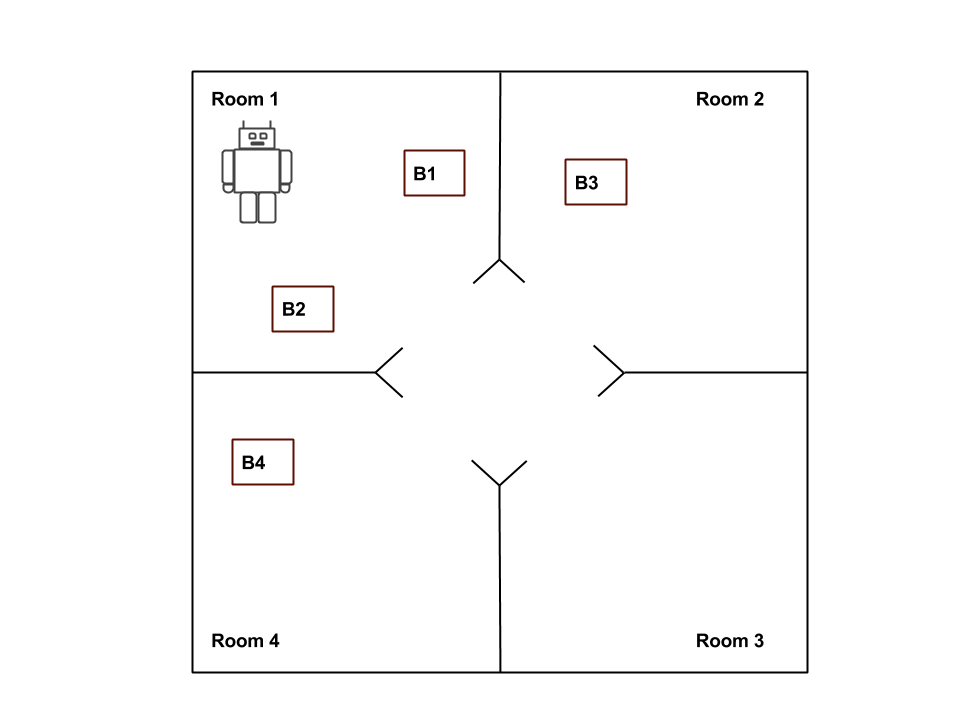
\includegraphics[width=10cm]{figures/salas.png}
  \caption{Estado para problema dos Robôs}
  \label{fig:salas}
\end{figure}

Usando o domínio dos robôs, rodamos experimentos para vinte diferentes estados iniciais e finais. Nos dez primeiros, tínhamos duas salas e número de caixas de um até dez (para cada novo teste, adicionávamos uma caixa). Todas as caixas estavam inicialmente em uma sala (Room 1) e como estado final deveriam estar na outra sala (Room 2).

Nos outros dez problemas, o número de salas também aumentou conforme aumentamos o número de caixas. Nestes problemas, cada caixa era posicionada inicialmente de tal forma que no estado final deveria estar na sala ao lado. Por exemplo, uma caixa inicialmente na sala 2 tem como meta estar na sala 3, uma caixa na sala 4 deve ir para 5 e assim por diante.

\subsubsection{Resultados}\label{problemas:robos:resultados}

%Grafico para time - Robos
\begin{figure}[H]
\centering
\begin{tikzpicture}
  \begin{axis}[
      only marks, xtick=data, xticklabels 
from table={plot/timeRobos2.dat}{Problema},
      xticklabel style={rotate=90},
      axis lines=left,
      xlabel={Problemas dos Robôs},
      xlabel style={at={(0.5,-0.1)}},
      ylabel={Tempo de Execução em milissegundos $log_{10}$},
      enlarge x limits={abs={0.0001*\pgfplotbarwidth}},
      legend style={at={(0.85,0.4)},anchor=north,legend columns=1},
      height=9cm, width=15cm]

      \addplot table [x expr=\coordindex, y=H0]{plot/timeRobos2.dat};
      \addplot table [x expr=\coordindex,
      y=GraphPlanHeuristic]{plot/timeRobos2.dat};
      \addplot table [x expr=\coordindex, 
      y=GraphPlanHeuristicOpt]{plot/timeRobos2.dat};
      \addplot table [x expr=\coordindex, 
      y=HSP_AddHeuristic]{plot/timeRobos2.dat};
      \addplot table [x expr=\coordindex, 
      y=HSP_MaxHeuristic]{plot/timeRobos2.dat};
  \legend{H0, Graph Plan, Graph Plan Otimo, HSP ADD, HSP MAX}
  \end{axis}
\end{tikzpicture}
\caption{Tempo de Execução - Problema dos Robôs}
\label{fig:tempoRobos}
\end{figure}




%Grafico para custo - Robos
\begin{figure}[H]
\centering
\begin{tikzpicture}
  \begin{axis}[
      only marks, xtick=data, xticklabels 
from table={plot/custoRobos.dat}{Problema},
      xticklabel style={rotate=90},
      axis lines=left,
      xlabel={Problemas dos Robôs},
      xlabel style={at={(0.5,-0.1)}},
      ylabel={Custo da Solução},
      enlarge x limits={abs={0.0001*\pgfplotbarwidth}},
      legend style={at={(0.85,0.4)},anchor=north,legend columns=1},
      height=9cm, width=15cm]

      \addplot table [x expr=\coordindex, y=H0]{plot/custoRobos.dat};
      \addplot table [x expr=\coordindex,
      y=GraphPlanHeuristic]{plot/custoRobos.dat};
      \addplot table [x expr=\coordindex, 
      y=GraphPlanHeuristicOpt]{plot/custoRobos.dat};
      \addplot table [x expr=\coordindex, 
      y=HSP_AddHeuristic]{plot/custoRobos.dat};
      \addplot table [x expr=\coordindex, 
      y=HSP_MaxHeuristic]{plot/custoRobos.dat};
  \legend{H0, Graph Plan, Graph Plan Otimo, HSP ADD, HSP MAX}
  \end{axis}
\end{tikzpicture}
\caption{Custo da Solução - Problema dos Robôs}
\label{fig:custoRobos}
\end{figure}


%Nos gerados e visitados Robos
\begin{table}[H]
\begin{tabular}{l|l|l|l|l|l|l|l|l|l|l|}
\cline{2-11}
                            & \multicolumn{2}{c|}{H0} & \multicolumn{2}{c|}{\begin{tabular}[c]{@{}c@{}}Graph \\ Plan\end{tabular}} & \multicolumn{2}{c|}{\begin{tabular}[c]{@{}c@{}}Graph \\ Plan \\ Optimo\end{tabular}} & \multicolumn{2}{c|}{\begin{tabular}[c]{@{}c@{}}HSP \\ ADD\end{tabular}} & \multicolumn{2}{c|}{\begin{tabular}[c]{@{}c@{}}HSP \\ MAX\end{tabular}} \\ \hline
\multicolumn{1}{|l|}{Prob.} & Visit.     & Ger.       & Visit                               & Ger.                                 & Visit.                                    & Ger.                                     & Visit.                              & Ger.                              & Visit.                              & Ger.                              \\ \hline
\multicolumn{1}{|l|}{2}     & 28         & 70         & 11                                  & 16                                   & 26                                        & 53                                       & 17                                  & 34                                & 17                                  & 34                                \\ \hline
\multicolumn{1}{|l|}{3}     & 297        & 1082       & 22                                  & 34                                   & 154                                       & 354                                      & 53                                  & 98                                & 53                                  & 98                                \\ \hline
\multicolumn{1}{|l|}{4}     & 3816       & 17549      & 37                                  & 58                                   & 928                                       & 2170                                     & 119                                 & 245                               & 119                                 & 245                               \\ \hline
\multicolumn{1}{|l|}{5}     & 58523      & 322124     & 56                                  & 88                                   & 4485                                      & 10168                                    & 269                                 & 618                               & 269                                 & 618                               \\ \hline
\multicolumn{1}{|l|}{6}     & -1         & -1         & 79                                  & 124                                  & 26019                                     & 56571                                    & 353                                 & 953                               & 353                                 & 953                               \\ \hline
\multicolumn{1}{|l|}{7}     & -1         & -1         & 106                                 & 166                                  & -1                                        & -1                                       & 537                                 & 1580                              & 537                                 & 1580                              \\ \hline
\multicolumn{1}{|l|}{8}     & -1         & -1         & -1                                  & -1                                   & -1                                        & -1                                       & -1                                  & -1                                & -1                                  & -1                                \\ \hline
\multicolumn{1}{|l|}{9}     & -1         & -1         & 172                                 & 268                                  & -1                                        & -1                                       & 1061                                & 3708                              & 1061                                & 3708                              \\ \hline
\multicolumn{1}{|l|}{10}    & -1         & -1         & 211                                 & 328                                  & -1                                        & -1                                       & 1438                                & 5389                              & 1438                                & 5389                              \\ \hline
\multicolumn{1}{|l|}{2B2R}  & 27         & 66         & 23                                  & 41                                   & 27                                        & 62                                       & 18                                  & 29                                & 18                                  & 29                                \\ \hline
\multicolumn{1}{|l|}{3B2R}  & 87         & 272        & 51                                  & 87                                   & 87                                        & 272                                      & 42                                  & 76                                & 42                                  & 76                                \\ \hline
\multicolumn{1}{|l|}{4B2R}  & 255        & 882        & 192                                 & 486                                  & 255                                       & 870                                      & 69                                  & 130                               & 69                                  & 130                               \\ \hline
\multicolumn{1}{|l|}{5B2R}  & 703        & 2612       & 603                                 & 1857                                 & 703                                       & 2612                                     & 158                                 & 319                               & 158                                 & 319                               \\ \hline
\multicolumn{1}{|l|}{6B2R}  & 1855       & 7214       & 1710                                & 5876                                 & 1855                                      & 7194                                     & 229                                 & 475                               & 229                                 & 475                               \\ \hline
\multicolumn{1}{|l|}{7B2R}  & 4735       & 19056      & 4537                                & 16707                                & 4735                                      & 19056                                    & 746                                 & 1666                              & 746                                 & 1666                              \\ \hline
\multicolumn{1}{|l|}{8B2R}  & 11775      & 48618      & 11516                               & 44450                                & 11775                                     & 48590                                    & 1017                                & 2290                              & 1017                                & 2290                              \\ \hline
\multicolumn{1}{|l|}{9B2R}  & 28671      & 120812     & 28343                               & 113157                               & 28671                                     & 120812                                   & 3890                                & 9305                              & 3890                                & 9305                              \\ \hline
\multicolumn{1}{|l|}{10B2R} & 68607      & 293862     & 68202                               & 279264                               & 68607                                     & 293826                                   & 5081                                & 12101                             & 5081                                & 12101                             \\ \hline
\end{tabular}
\caption{Nós Visitados e Gerados - Problema dos Robôs}
\label{tab:nosRobos}
\end{table}

Na figura \ref{fig:tempoRobos} podemos observar que a heurística GraphPlan foi a que produziu tempos menores seguida de HSPAdd, conseguindo resolver problemas mais difíceis, para as instâncias onde o robô tem que deixar as caixas em outros quartos. Já o HSPMax, e o H0 foi os que tiveram o pior comportamento: foi o que mais demorou para devolver uma solução e o que resolveu a menor quantidade de problemas.

Na segunda parte do problema, onde os robôs tem de deixar as caixas no quarto 2, o GraphPlan produziu os piores resultados, em parte devido ao tempo de computação da heurística. O H0, produziu os melhores resultados precisamente por isso.

A tabela \ref{fig:custoBlocos} apresenta o custo das soluções encontradas.
O custo mínimo vem dado pelo uso da heurística H0 que é admissível.
O GraphPlan e o HSPAdd são heurísticas não admissíveis e as soluções encontradas tem um custo maior.